\documentclass{article}

\usepackage[margin=2.5cm,left=2cm,includefoot]{geometry}
\usepackage{graphicx}
\usepackage{float}
\usepackage[space]{grffile}
\usepackage{hyperref}
\usepackage[export]{adjustbox}
\usepackage{multicol}
\usepackage{caption}
\usepackage{hyperref}
\usepackage{listings}
\usepackage{vhistory}
\usepackage{titlesec}

\setcounter{secnumdepth}{4}

\titleformat{\paragraph}
{\normalfont\normalsize\bfseries}{\theparagraph}{1em}{}
\titlespacing*{\paragraph}
{0pt}{3.25ex plus 1ex minus .2ex}{1.5ex plus .2ex}

% Header and footer
\usepackage{fancyhdr}
\pagestyle{fancy}

\rhead{COS301}
\lhead{Testing Document}
\fancyfoot[R]{Page \thepage}

\renewcommand{\headrulewidth}{2pt}
\renewcommand{\footrulewidth}{1pt}

\begin{document}

	\begin{titlepage}
		\begin{center}
			
\includegraphics[width=10cm]{images/UP.jpg}  \\
			[0.5cm]
			\huge{
			Test Plan and Report\\
			}
			
			\line(1,0){300}\\
			[0.2cm]
			\LARGE{Project: Insurance profiling from social media\\
			Client: RetroRabbit} \\
			\line(1,0){300}\\
			\LARGE{Team: Valknut Solutions}\\
			[1.0cm]
			\large{Version: 1.1}\\
			[1.0cm]
			\large
			{
			\begin{itemize}
				\item 13054903 - Charl Jansen van Vuuren    
				\item 13044924 - Kevin Heritage
				\item 13176545 - Quinton Weenink\\
			\end{itemize}
			}
			\textsc{\large}\\
		[3.0cm]
		\textsc{\large  Department of Computer Science}\\
		[0.5cm]
		\textsc{\large \today}\\
		\end{center}
	\end{titlepage}
	
	\cleardoublepage
	% Start of the revision history table
	\begin{versionhistory}
  		\vhEntry{1.0}{27.7.2016}{CJvV,KH,QW}{created}
  		\vhEntry{1.1}{04.9.2016}{CJvV,KH,QW}{Updated format based on template on CS web, added new test information}
	\end{versionhistory}	
	
	\cleardoublepage
	\tableofcontents
	\cleardoublepage
	
\section{Introduction}
This document contains information related to Testing of the Insurance Profiling project that is being developed for RetroRabbit as part of the COS301 module at the University Of Pretoria. \\
This document is based on the IEEE 829 Standard for Testing Documentation \href{http://www.fit.vutbr.cz/study/courses/ITS/public/ieee829.html}{IEEE 829}
The structure of this document includes an initial scope and purpose, a Unit test plan and the final Unit test report.
\subsection{Purpose}
This document combines the unit test plan and report into a single coherent artefact. The overall purpose of the system is to allow the analysis of different social media inputs (Facebook in particular) by means of a marketing and risk analysis standpoint.
Test driven development is crucial to our system as it ensures every added feature is compatible with the current version of the system and that feature is working as intended.
\subsection{Scope}
The scope of this document is structured as follows. The features that are considered for testing are listed as per section \ref{sec:testItems}. \\
Tests that have been identified from the requirements are
discussed in detail in section \ref{sec:FeaturesTest}.\\
Furthermore, this document outlines the test environment and the risks involved in the testing approaches that will be followed as per section \ref{subsec:testEnvironment}. Assumptions and dependencies of this test plan will also be mentioned as per section \ref{subsec:assumptions} . Section ... , ... and ...  outlines, discusses and concludes on the results of the tests, respectively.
\subsection{Test Environment}\label{subsec:testEnvironment}
The testing environment is mainly software based and includes:
\begin{itemize}
	\item Programming languages:
	\begin{itemize}
		\item Javascript 
	\end{itemize}
	\item Testing Frameworks:
	\begin{itemize}
		\item MochaJS - Unit tests
		\item Travis CI - Continuous integration for deployment
	\end{itemize}
	\item Coding Environment:
	\begin{itemize}
		\item NodeJS based web server
		\item ExpressJS
		\item PostgreSQL database with Sequelize ORM
		\item Terminal based test outputs
	\end{itemize}
	\item Operating system:
	\begin{itemize}
		\item Ubuntu Linux
		\item Microsoft Windows 10
	\end{itemize}
	\item Internet Browsers:
	\begin{itemize}
		\item Mozilla Firefox
		\item Chrome web browser
	\end{itemize}
\end{itemize}

\subsection{Assumptions and Dependencies}\label{subsec:assumptions}
Assumptions:
\begin{itemize}
	\item 
\end{itemize}
Dependencies:
\begin{itemize}
	\item
\end{itemize}


\section{Test items}\label{sec:testItems}
\subsection{The items included in this test document includes:}
\begin{itemize}
	\item Backend API calls
	\item Database management functions
	\item Environmental tests 
	\item Deployment and compatibility tests
\end{itemize} 

\section{Functional Features to be Tested}\label{sec:FeaturesTest}
Test estimation can be categorized as fast (nearly instant tests) or slow (timely tests with external dependencies) for our system. \\ 
\subsection{Overall approach with regards to adequate testing of :} 
\begin{itemize}
\item Feature unit tests:
\begin{itemize}
	\item Mocking out the non essential dependencies to be able to test the feature
	\item Include the essential dependencies that cannot be mocked out
	\item Estimation of this feature group can be concluded as "fast".
\end{itemize}
\item Backend API tests:
\begin{itemize}
	\item Estimation of this feature group can be concluded as "slow" as it is dependent on the external server.
\end{itemize}
\item Environmental tests:
\begin{itemize}
	\item Estimation of this feature group can be concluded as "fast" as it is a simple check for current environment.
\end{itemize}
\item Deployment tests:
\begin{itemize}
	\item Estimation of this feature group can be concluded as "slow" as it is dependent on the external Travis CI server.
\end{itemize}
\end{itemize}

\subsection{The included features to be tested:}
\begin{itemize}
\item Feature unit tests:
	\begin{itemize}
	\item The ability to receive data from a Facebook lead ad and save this data in the database.
	\item The ability to receive data from any other integration point as per the specified format.
	\item These feature relates to the getLeadData use case in the Functional requirements documentation
	\end{itemize}
\item API calls to do:
	\begin{itemize}
	\item Database insertions 
	\item Database deletions 
	\item Database retrievals 
	\item This test relates to the Analysis use case in the Functional requirements documentation, it forms the underlying persistence with regards to the data analysis is done on.
	\end{itemize}
\item Environmental test
	\begin{itemize}
	\item Integration test to determine the current environment (development or deployment) to react accordingly 
	\end{itemize}
\item Deployment/Build testing including Compatibility
		\begin{itemize}
	\item Automated testing by the Travis CI framework to ensure the current feature is compatible with different versions of the NodeJS framework. 
	\end{itemize}
\end{itemize}

\begin{table}[]
\centering
\caption{Test cases}
\label{test_table}
\begin{tabular}{|l|l|l|l|}
\hline
Feature ID & RDS Source                            & Summary                                    & Test Case ID \\ \hline \hline
1          & Functional requirements - getLeadData & Receive data from a Facebook lead ad       & 1            \\ \hline
2          & Functional requirements - getLeadData    & Receive data from other integration source & 2            \\ \hline
3          & Functional requirements - Analysis    & Database insertions                        & 3            \\ \hline
4          & Functional requirements - Analysis    & Database deletions                         & 4            \\ \hline
5          & Functional requirements - Analysis    & Database retrievals                        & 5            \\ \hline
6          &  Architecture design - Section 5      & Environmental test                         & 6            \\ \hline
7          &  Architecture design - Section 5.1.1  & Deployment test                            & 7            \\ \hline
\end{tabular}
\end{table}


\section{Test instructions} %TODO : onwards %
Tests can be ran with the command "npm test" which will run Mocha, if this test is run locally it will connect to the local database.
Travis CI runs these test to the external database hosted on Heroku. The Travis tests are ran when a new branch is merged to ensure compatibility with all versions of Node.
\section{Item Pass/Fail Criteria for Tests}
If the specified Pre-condition is not met the test will fail. \\
If the specified Post-condition is met the test will pass.
\cleardoublepage
\section{Test cases}
\subsection{The following tests all passed as intended:}
\begin{itemize}
\item Creating row in Database - POST : /api/user/ 
	\begin{itemize}
	\item Pre-conditions:
		\begin{itemize}
		\item Database is connected and created
		\item The following values are specified:  
		\begin{itemize}
		\item firstName
  		\item lastName
  		\item mobileNumber 
  		\item maritalStatus 
  		\item dateOfBirth 
 		\item gender
  		\item location 
 		\item email
 		\end{itemize} 
		\end{itemize}
	\item Post-condition - The row gets persisted
	\item Figure \ref{fig:MochaTests}
	\end{itemize}

\item Retrieving row in Database based on currentUser - GET : /api/user/:currentUser
	\begin{itemize}
	\item Pre-condition - The currentUser exists
	\item Post-condition - The currentUser is retrieved 
	\item Figure \ref{fig:MochaTests}
	\end{itemize}
	
\item Removing row in Database based on currentUser - DELETE : /api/user/:currentUser
	\begin{itemize}
	\item Pre-condition - The currentUser exists
	\item Post-condition - The currentUser is removed 
	\item Figure \ref{fig:MochaTests}
	\end{itemize}	
	\begin{figure}[H]
  	\centering
      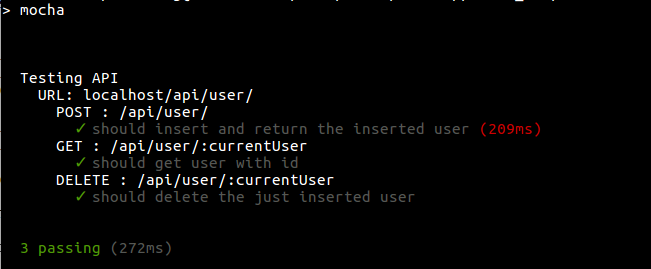
\includegraphics[width=\textwidth]{images/tests.png}
  	\caption{Output of Mocha tests}
  	\label{fig:MochaTests}
	\end{figure}


\item Travis CI build test for Node version 5.11
	\begin{itemize}
	\item Pre-condition - The changes to the branch are compatible with version 5.11
	\item Post-condition - The build will pass successfully 
	\item Figure \ref{fig:5_11}
	\end{itemize}	
	
	\begin{figure}[h]
  	\centering
      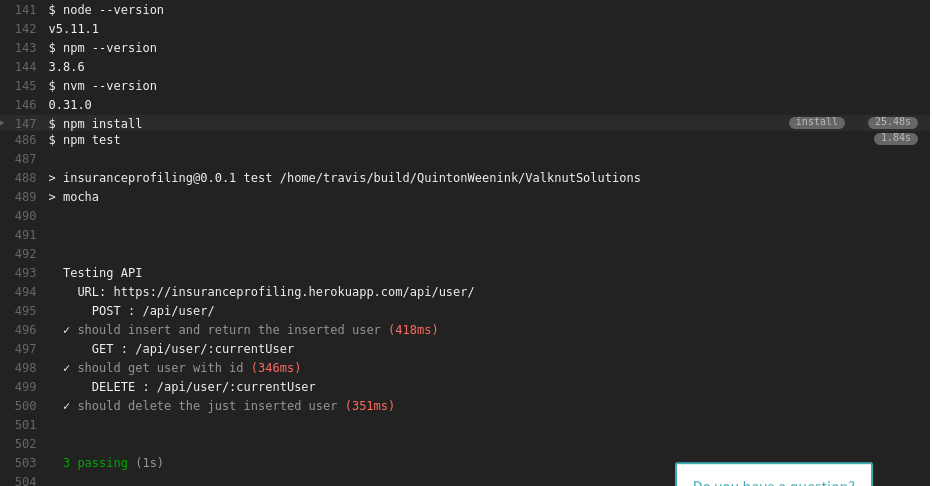
\includegraphics[width=\textwidth]{images/5_11.png}
  	\caption{Output of Travis tests for Node version 5.11}
  	\label{fig:5_11}
	\end{figure}

\cleardoublepage
\item Travis CI build test for Node version 6.2
	\begin{itemize}
	\item Pre-condition - The changes to the branch are compatible with version 6.2
	\item Post-condition - The build will pass successfully 
	\item Figure \ref{fig:6_2}
	\end{itemize}	
\end{itemize}

\begin{figure}[h]
  \centering
      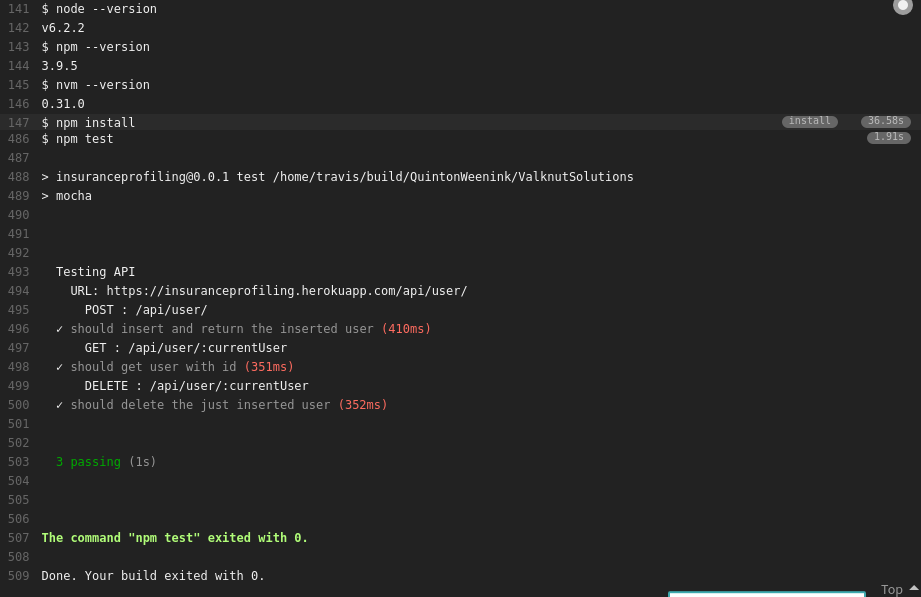
\includegraphics[width=\textwidth]{images/6_2.png}
  \caption{Output of Travis tests for Node version 6.2}
  \label{fig:6_2}
\end{figure}


\cleardoublepage
\subsection{The following tests failed as intended:}
\begin{itemize}
	\item Travis CI build, running Mocha when a branch was merged.
	\begin{itemize}
	\item Pre-condition - Heroku server is online.
	\item Post-condition - The build will pass successfully 
	\item Figure \ref{fig:failed}
	\item This test failed as a result of the hosting server being offline, not fulfilling the Pre-condition. 
	\item The error stating a timeout proves this failure.
	\end{itemize}

	\begin{figure}[h]
  	\centering
      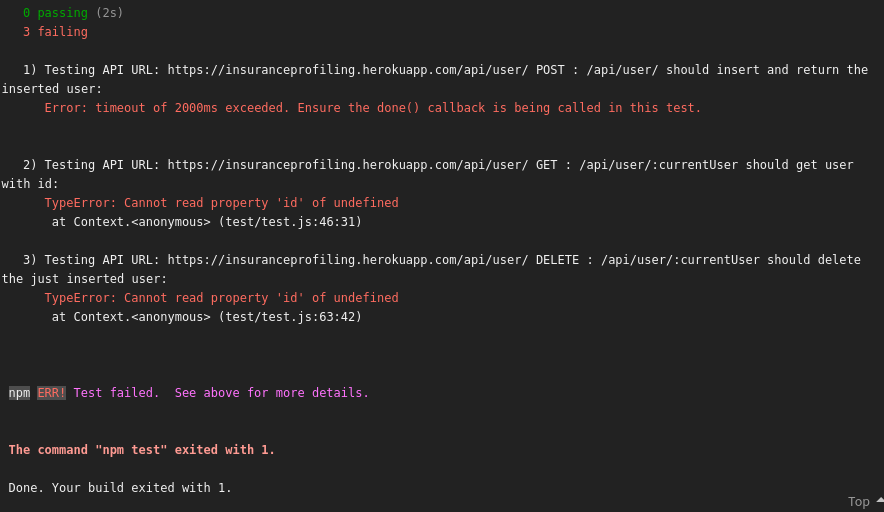
\includegraphics[width=\textwidth]{images/failed.png}
  	\caption{Output of failed Travis test}
  	\label{fig:failed}
	\end{figure}	
	
	\cleardoublepage
	\item Database connection test based on Mocha test
	\begin{itemize}
	\item Pre-conditions
	\begin{itemize}
		\item The database exists and is created
		\item The database accepts connections
	\end{itemize}
	\item Post-condition - The test will pass
	\item Figure \ref{fig:DBFailed}
	\item This test failed as a the Pre-conditions did not hold. 
	\item The database was not initialized at that time.
	\end{itemize}


	\begin{figure}[h]
  	\centering
      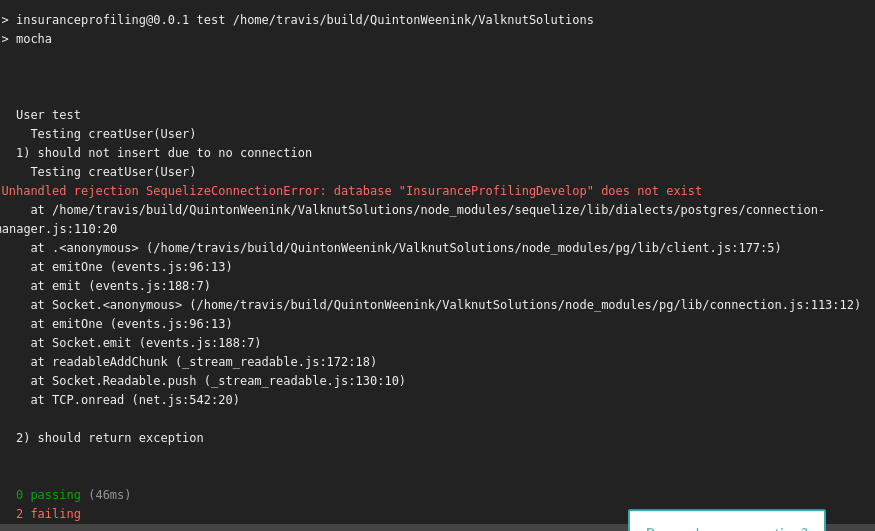
\includegraphics[width=\textwidth]{images/DBConnectionFailed.png}
  	\caption{Database connection test}
  	\label{fig:DBFailed}
	\end{figure}	
	
	
	\begin{figure}[h]
  	\centering
      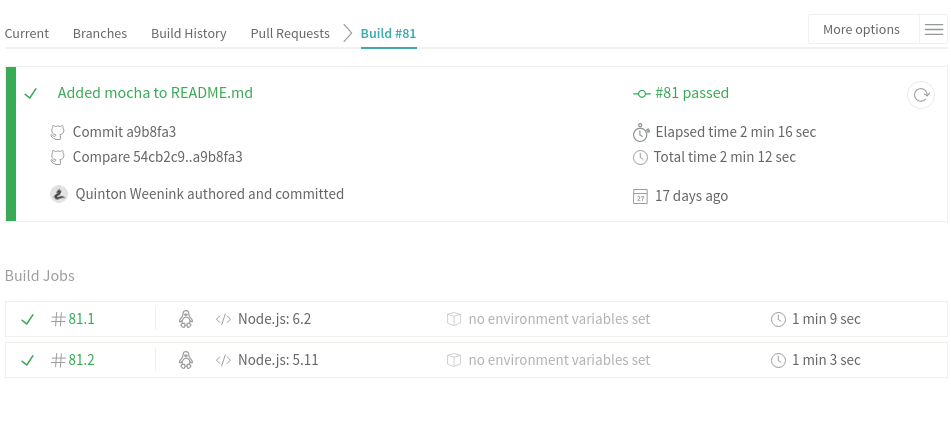
\includegraphics[width=\textwidth]{images/TravisInterface.png}
  	\caption{Travis interface used for test logs}
	\end{figure}

\end{itemize}

\cleardoublepage
\section{Test Summary}
This project follows a Continous Integration model with regards to testing. \\ Any new feature to be merged with the main branch is first tested, then reviewed by the person merging the branch and only then the merge is closed.\\
The amount of tests are limited in the current version of the system, this is as a result of the complexity of testing external API calls,such as Facebook, on which our system heavily relies.\\
Future versions will include more tests based on these complexities.

\end{document}
